% Created 2016-03-08 Tue 19:26
\documentclass[11pt]{article}
\usepackage[utf8]{inputenc}
\usepackage[T1]{fontenc}
\usepackage{fixltx2e}
\usepackage{graphicx}
\usepackage{longtable}
\usepackage{float}
\usepackage{wrapfig}
\usepackage{rotating}
\usepackage[normalem]{ulem}
\usepackage{amsmath}
\usepackage{textcomp}
\usepackage{marvosym}
\usepackage{wasysym}
\usepackage{amssymb}
\usepackage{hyperref}
\tolerance=1000
\usepackage{color}
\usepackage{minted}
\usepackage{color}
\usepackage{minted}
\usepackage{parskip}
\author{Tammo Rukat}
\date{March 10, 2016}
\title{The Hamming Machine}
\hypersetup{
  pdfkeywords={},
  pdfsubject={},
  pdfcreator={Emacs 24.5.1 (Org mode 8.2.10)}}
\begin{document}

\maketitle
\setcounter{tocdepth}{1}
\tableofcontents


\section*{Basics}
\label{sec-1}
\begin{itemize}
\item Based on the hamming distance between two binary vectors ${h(\mathbf{x},\mathbf{u})}$ we construct a probability distribution of ${\mathbf{x}}$ given ${\mathbf{u}}$ with a dispersion parameter ${\lambda}$: $$ p(\mathbf{x}|\mathbf{u}) \propto \exp\left[ -\lambda h(\mathbf{x},\mathbf{u}) \right] $$
\item We assume a set of ${M}$ binary vectors ${\mathbf{u}_{1\ldots M}}$, that we call \textbf{codes}.
\item Each observations ${\mathbf{x} }$ is generated from a subset of these codes: $$ p(\mathbf{x}|\mathbf{U},\mathbf{s},\lambda) \propto \prod\limits_m p(\mathbf{x}|\mathbf{u}_m,\lambda)^{s_m} = \prod\limits_d \exp\left[ \sum_m s_m \lambda h(x_d,u_{md}) \right]$$
\item We find the normalised probability to be sigmoidal: $$ p(x_d = 1|\mathbf{s}, \mathbf{U}, \lambda) = \frac{1}{1+\exp\left[ \lambda \sum_m s_m (2u_{md} - 1) \right]} $$
\end{itemize}

\section*{Sigmoid Belief Net}
\label{sec-2}
\begin{itemize}
\item $$ p(x_d = 1|\mathbf{s}, \mathbf{U}, \lambda) =\frac{1}{1+\exp\left[ \lambda \sum_m s_m (2u_{md} - 1) \right]} $$
\end{itemize}


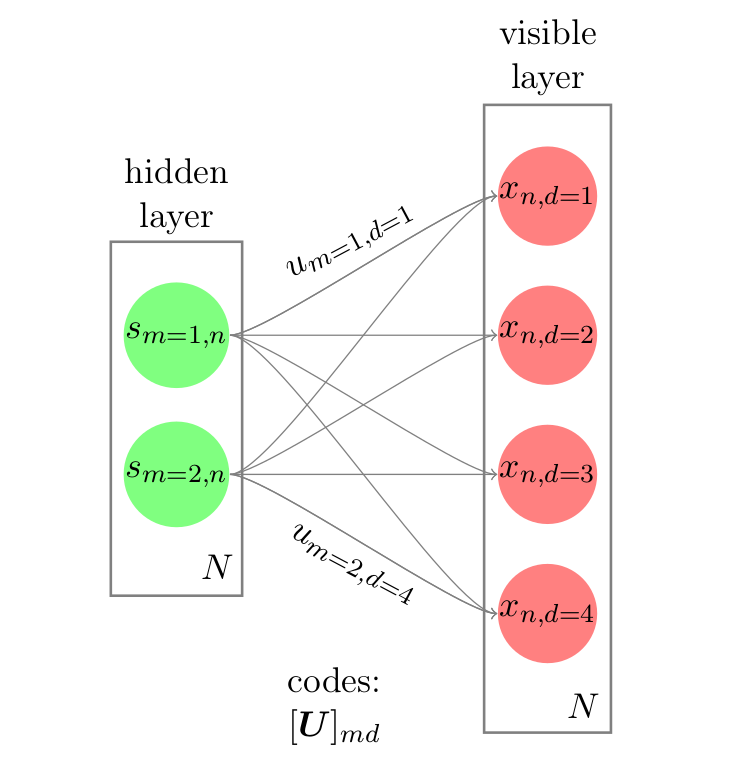
\includegraphics[width=.9\linewidth]{figures/hm0_1.png}

\section*{Inference}
\label{sec-3}
\begin{itemize}
\item Gibbs sampling for ${\mathbf{u}}$ and ${\mathbf{s}}$ with uninformative priors.
\item Metropolis Hastings for $\lambda$ with inverse gamma prior.
\item Precomputing quantities of the form $$ \log(1+e^{-\lambda m}); \,\,\,\, \text{for} \, m \in \{-M,\ldots,-1,0,1,\ldots,M\} $$ speeds up the computation.
\end{itemize}

\section*{Multilayer Hamming Machine}
\label{sec-4}
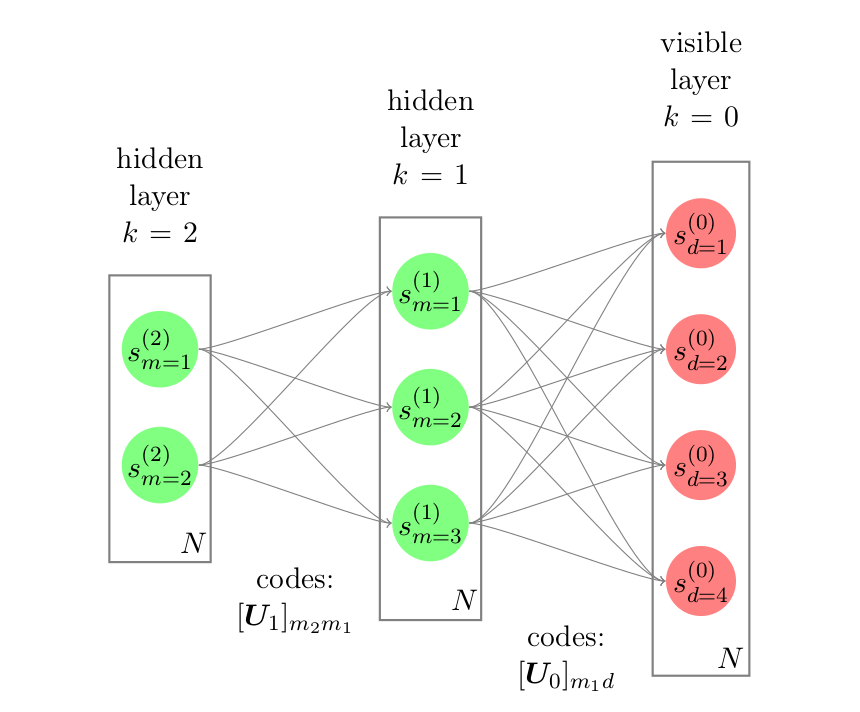
\includegraphics[width=.9\linewidth]{figures/hm2.png}
\begin{itemize}
\item The lower layer acts like a prior on the peripheral layer.
\end{itemize}

\section*{Toy Example}
\label{sec-5}
\url{figures/a4_10_5.gif}

\section*{Sparsity priors on ${\mathbf{u}}$}
\label{sec-6}
\begin{enumerate}
\item Independent Bernoulli prior on every single code unit ${u_{md}}$
\item Bernoulli prior controlling the number of 1s in every code.
\end{enumerate}
E.g. \emph{step-exp prior}

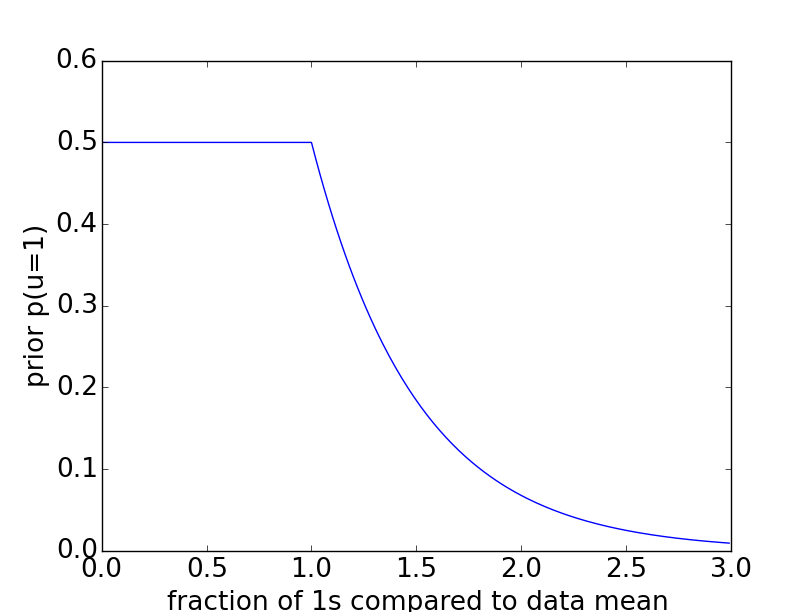
\includegraphics[width=.9\linewidth]{figures/prior.png}
$$  p(u = 1) = \tfrac{1}{2} \mathrm{H}( 1 - q ) + \tfrac{1}{2} \mathrm{H}(q-1) e^{-a(q-1)} $$

\subsection*{Effect of sparsity prior}
\label{sec-6-1}
\url{figures/a4_10_5_sparse.gif}

\section*{Example -- mnist}
\label{sec-7}
\subsection*{Sampling}
\label{sec-7-1}
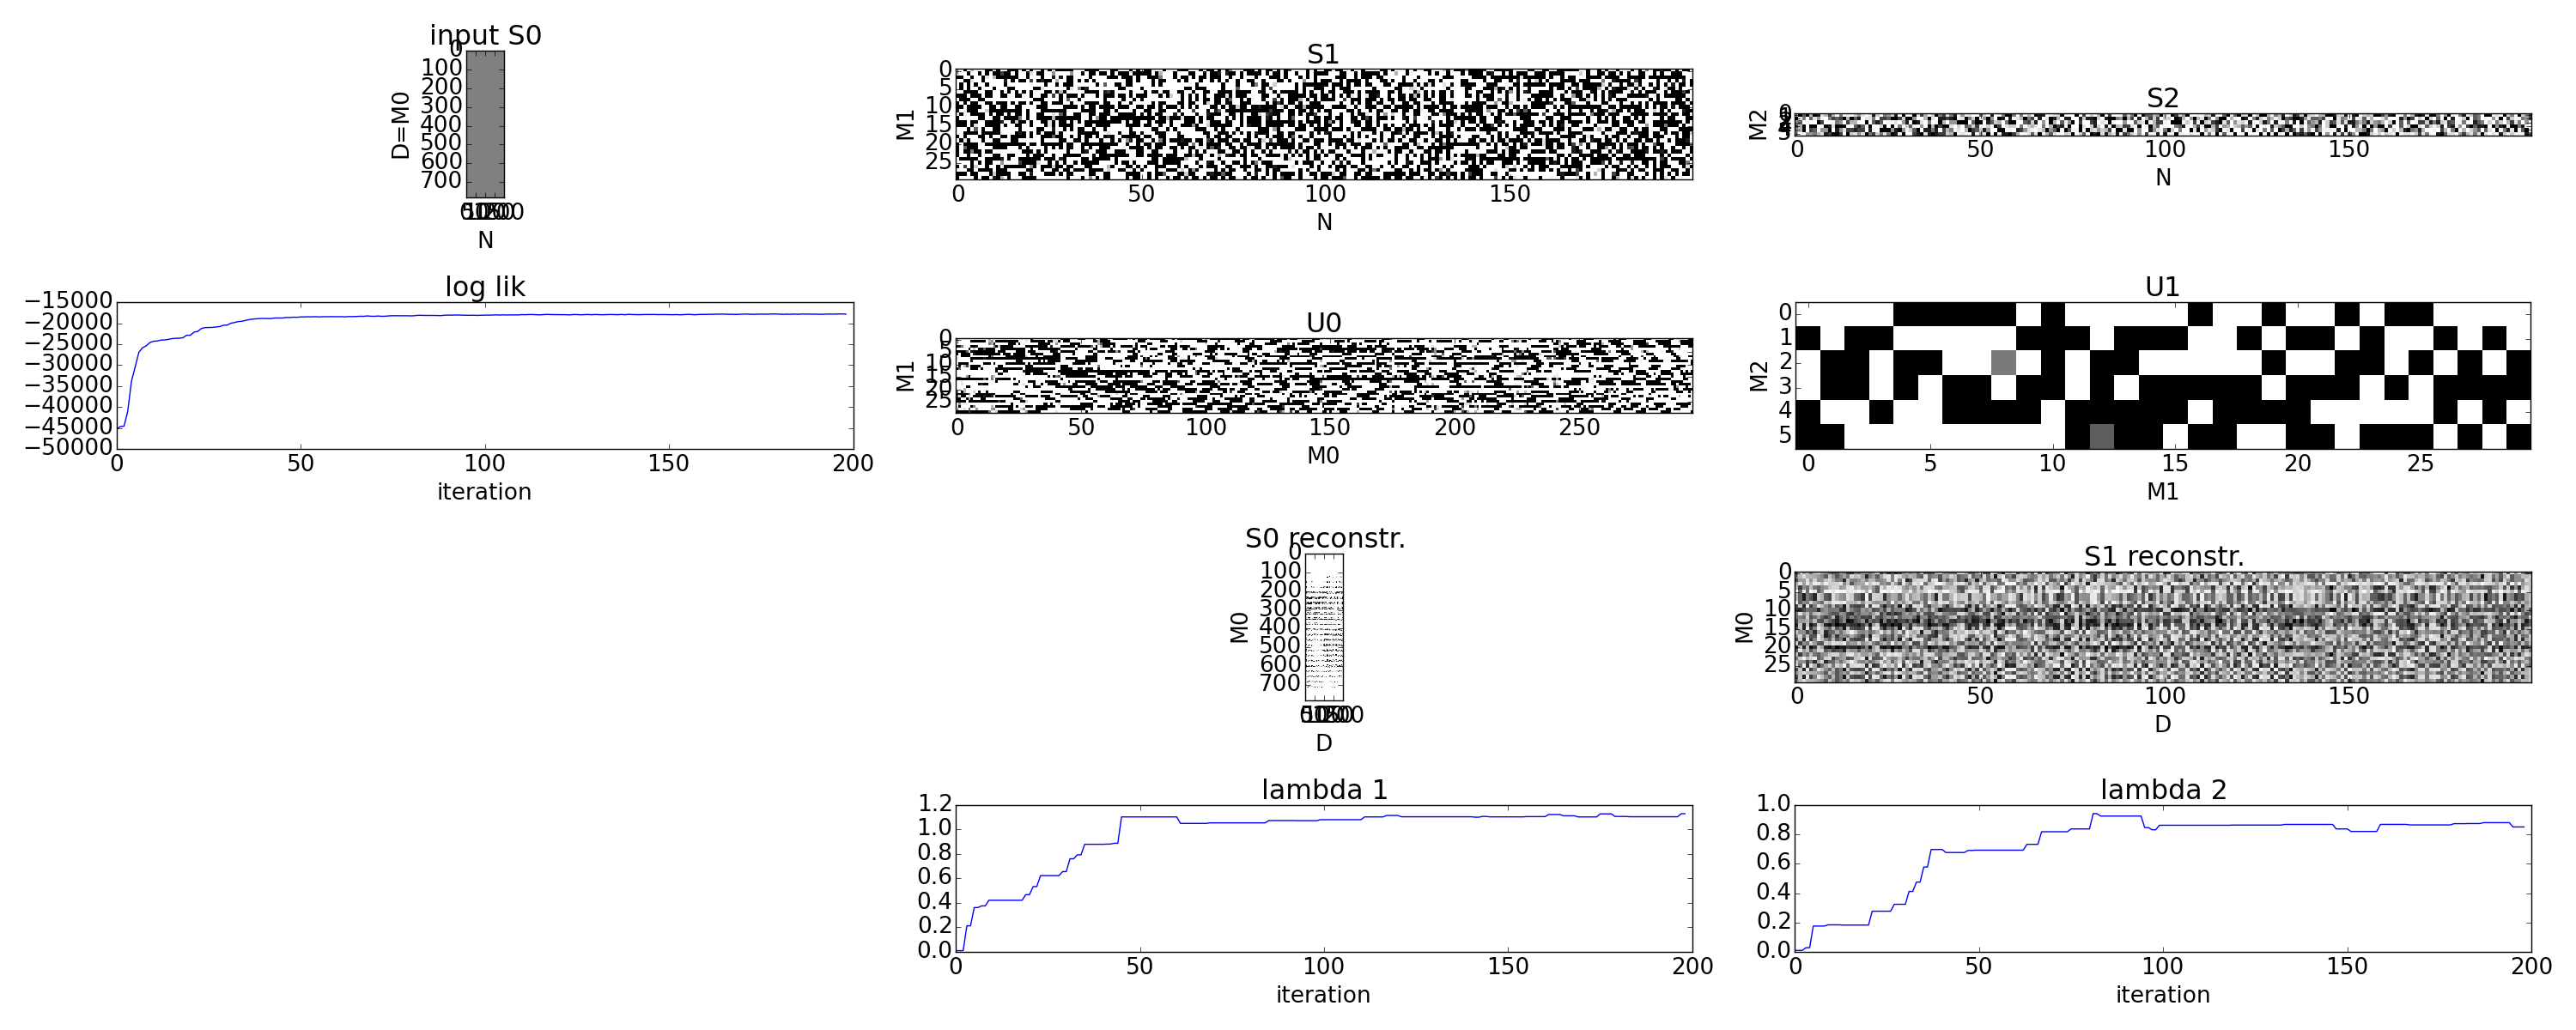
\includegraphics[width=.9\linewidth]{figures/mnist_sampler.png}
\subsection*{Reconstructions}
\label{sec-7-2}
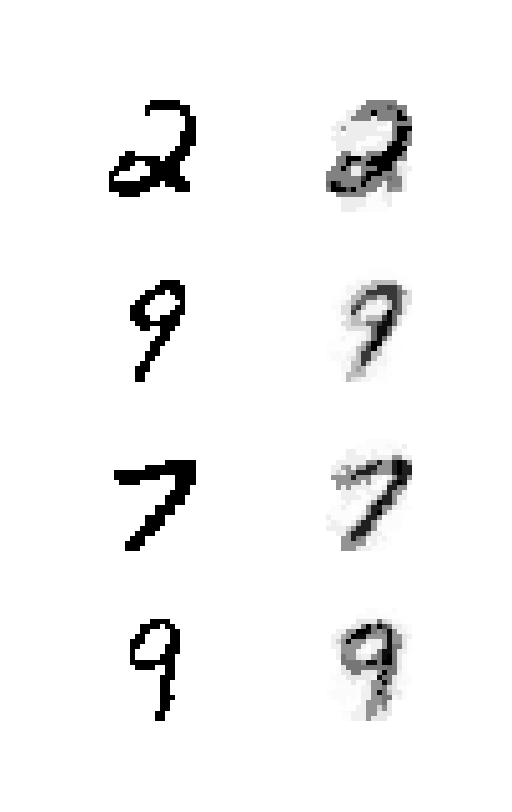
\includegraphics[width=.9\linewidth]{figures/recon_1.png}
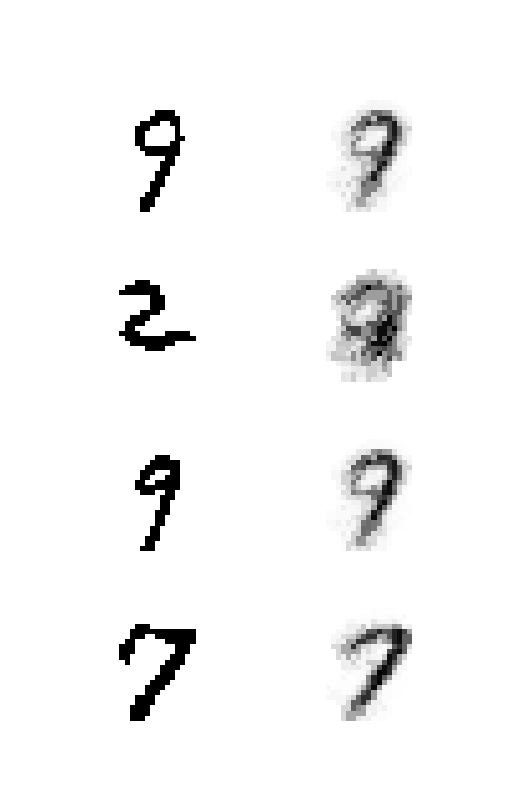
\includegraphics[width=.9\linewidth]{figures/recon_2.png}
\subsection*{Patterns}
\label{sec-7-3}
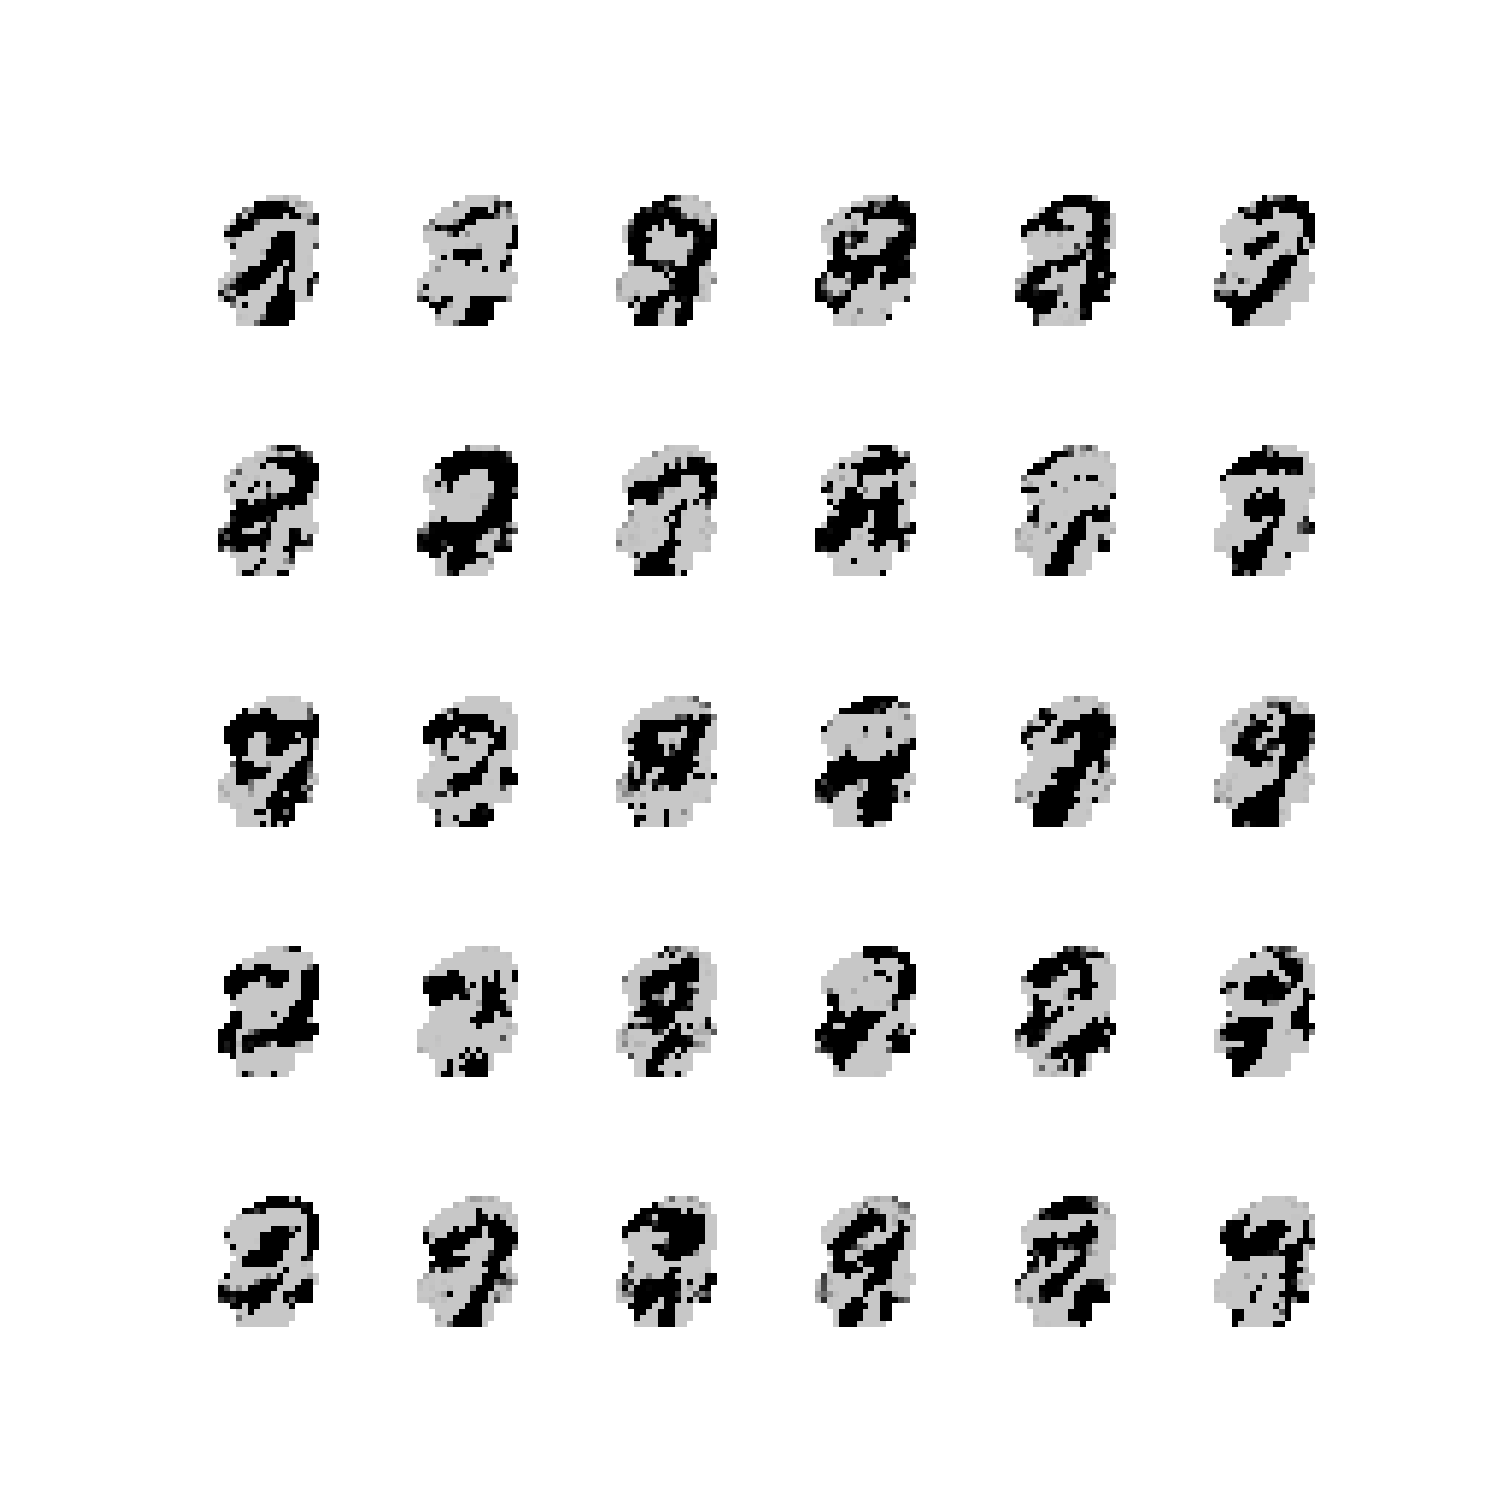
\includegraphics[width=.9\linewidth]{figures/snb_1_1.png}
\subsection*{Patterns}
\label{sec-7-4}
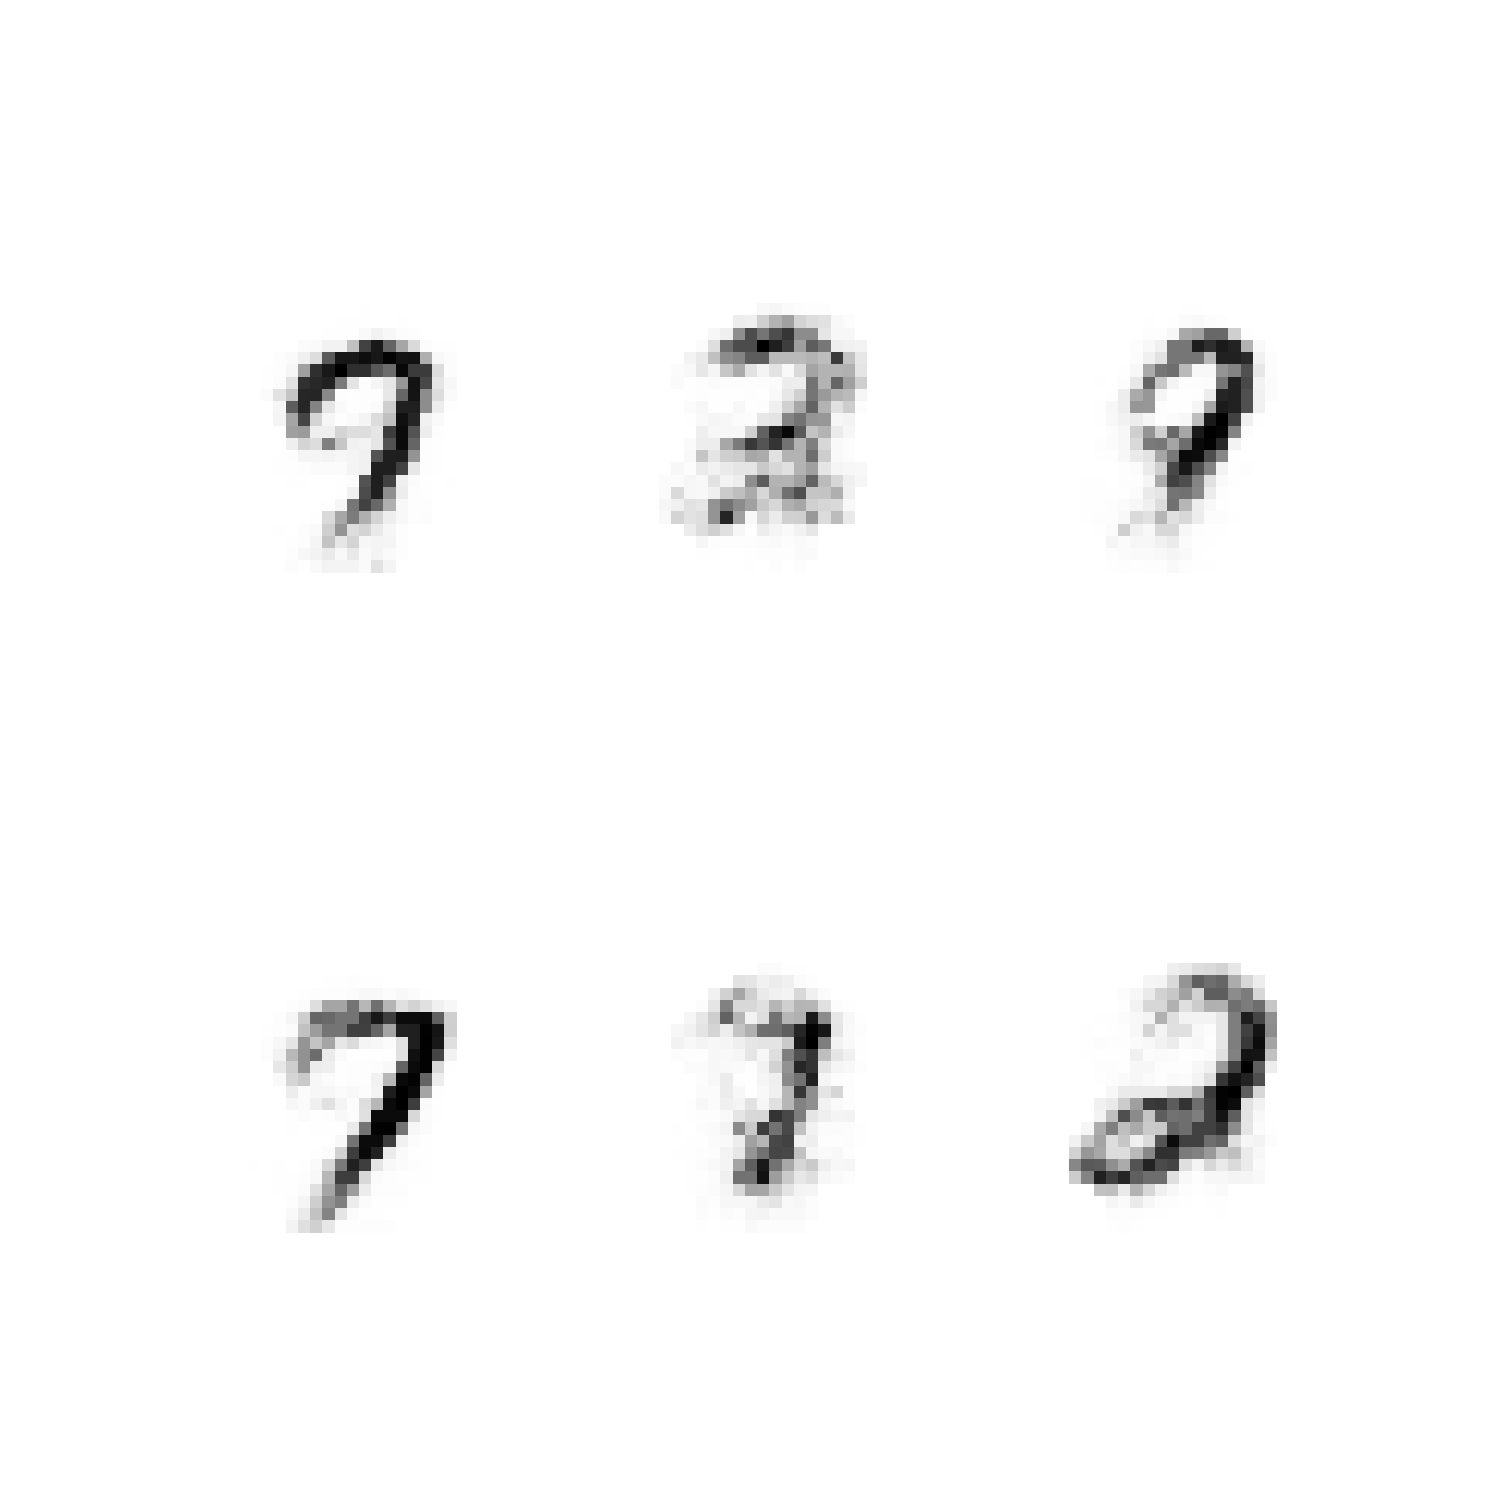
\includegraphics[width=.9\linewidth]{figures/snb_0_1.png}
% Emacs 24.5.1 (Org mode 8.2.10)
\end{document}